\section{YouTube-VOS Challenge 2022}
\label{sec:rvos_ytvos}
The YouTube-VOS Challenge provides a large-scale dataset for video object segmentation tasks, allowing us to design an algorithm to solve the long-term spatial-temporal dependency explicitly. Since 2018, it has been organized every year except the year of 2020. The challenge has introduced three challenges for different video object segmentation tasks, including:
\begin{itemize}
    \item Semi-supervised Video Object Segmentation
    \item Video Instance Segmentation
    \item Referring Video Object Segmentation
\end{itemize}

In 2022, The 4th Large-scale Video Object Segmentation Challenge was held as a workshop in conjunction with CVPR 2022, New Orleans, Lousiana. In the Video instance segmentation tasks, there is an extend of long video for validation and testing. 
% We participated in the Track 3: Referring Video Object Segmentation to experiment our method 

\subsection{Dataset}
The dataset was created based on the YouTube-VOS-2019 dataset, called Refer-YouTube-VOS. 
The Refer-Youtube-VOS contains 3,978 high-resolution YouTube videos with 131k high-quality manual annotations and 15k language expressions. The dataset is divided into 3,471 training videos, 202 validation videos, and 305 test videos.

\subsection{Evaluation metrics}
The region similarity($\mathcal{J}$) and contour accuracy($\mathcal{F}$) are used as the evaluation metrics for this challenge. The final ranking is sorted according to the average between these two metrics. 
\label{sec:metric}
\begin{itemize}
    \item \textbf{Region similarity $\mathcal{J}$} - To measure the similarity of region-based segmentation, i.e., the number of correct pixels and mislabeled pixels, the Jaccard index $\mathcal{J}$ is used. The Jaccard index, also known as the IoU metric, is to quantify the percent overlap between the target mask and our prediction. For simplification, the Jaccard index can be calculated by the division of the number of common pixels between the target mask and the prediction over the total number of pixels appearing across both masks. Given an output segmentation $P$ and the ground-truth mask $G$, it is defined as  

\begin{equation}
    \mathcal{J} = \frac{|P \cap G|}{|P \cup G|}
\end{equation}

with $|X|$ is the area of that segmentation. 
    \item \textbf{ Contour accuracy $\mathcal{F}$} - From a contour-based perspective, we can consider a segmentation $P$ as a set of closed contours $c(P)$ which delimits the spatial extent of the mask. We can compute the contour-based precision $P_c$ and recall $R_c$ between the contour points $c(P)$ and $c(G)$ of the output segmentation and ground-truth, respectively, via a bipartite graph matching in order to maximize the accuracies. The F-measure $\mathcal{F}$ is used as a good trade-off between precision and recall, defined as 
\begin{equation}
    \mathcal{F} = \frac{2P_c R_c}{P_c + R_c}
\end{equation}
\end{itemize}

\subsection{Implementation details}
We used Detectron2 to train our network. The text encoder is frozen during the training stage. In the Transformer Decoder, we choose L = 2 with 6 decoder layers in total. The initial backbone weights have been previously pretrained on YouTube-VIS 2021 from Mask2Former \cite{cheng_masked-attention_2022}. STCN is pretrained mainly on saliency datasets and finetuned over training splits of semi-supervised VOS tasks.
We train the network for 100k iterations using the AdamW optimizer with the initial learning rate $10^{−4}$. A factor of 0.1 decreases the learning rate at the $70.000$-th iteration. We train the network with a small batch size of 2 on 2 Tesla V100 with 16GB GPU.

\subsection{Results}


\begin{table}[ht]
    \centering
    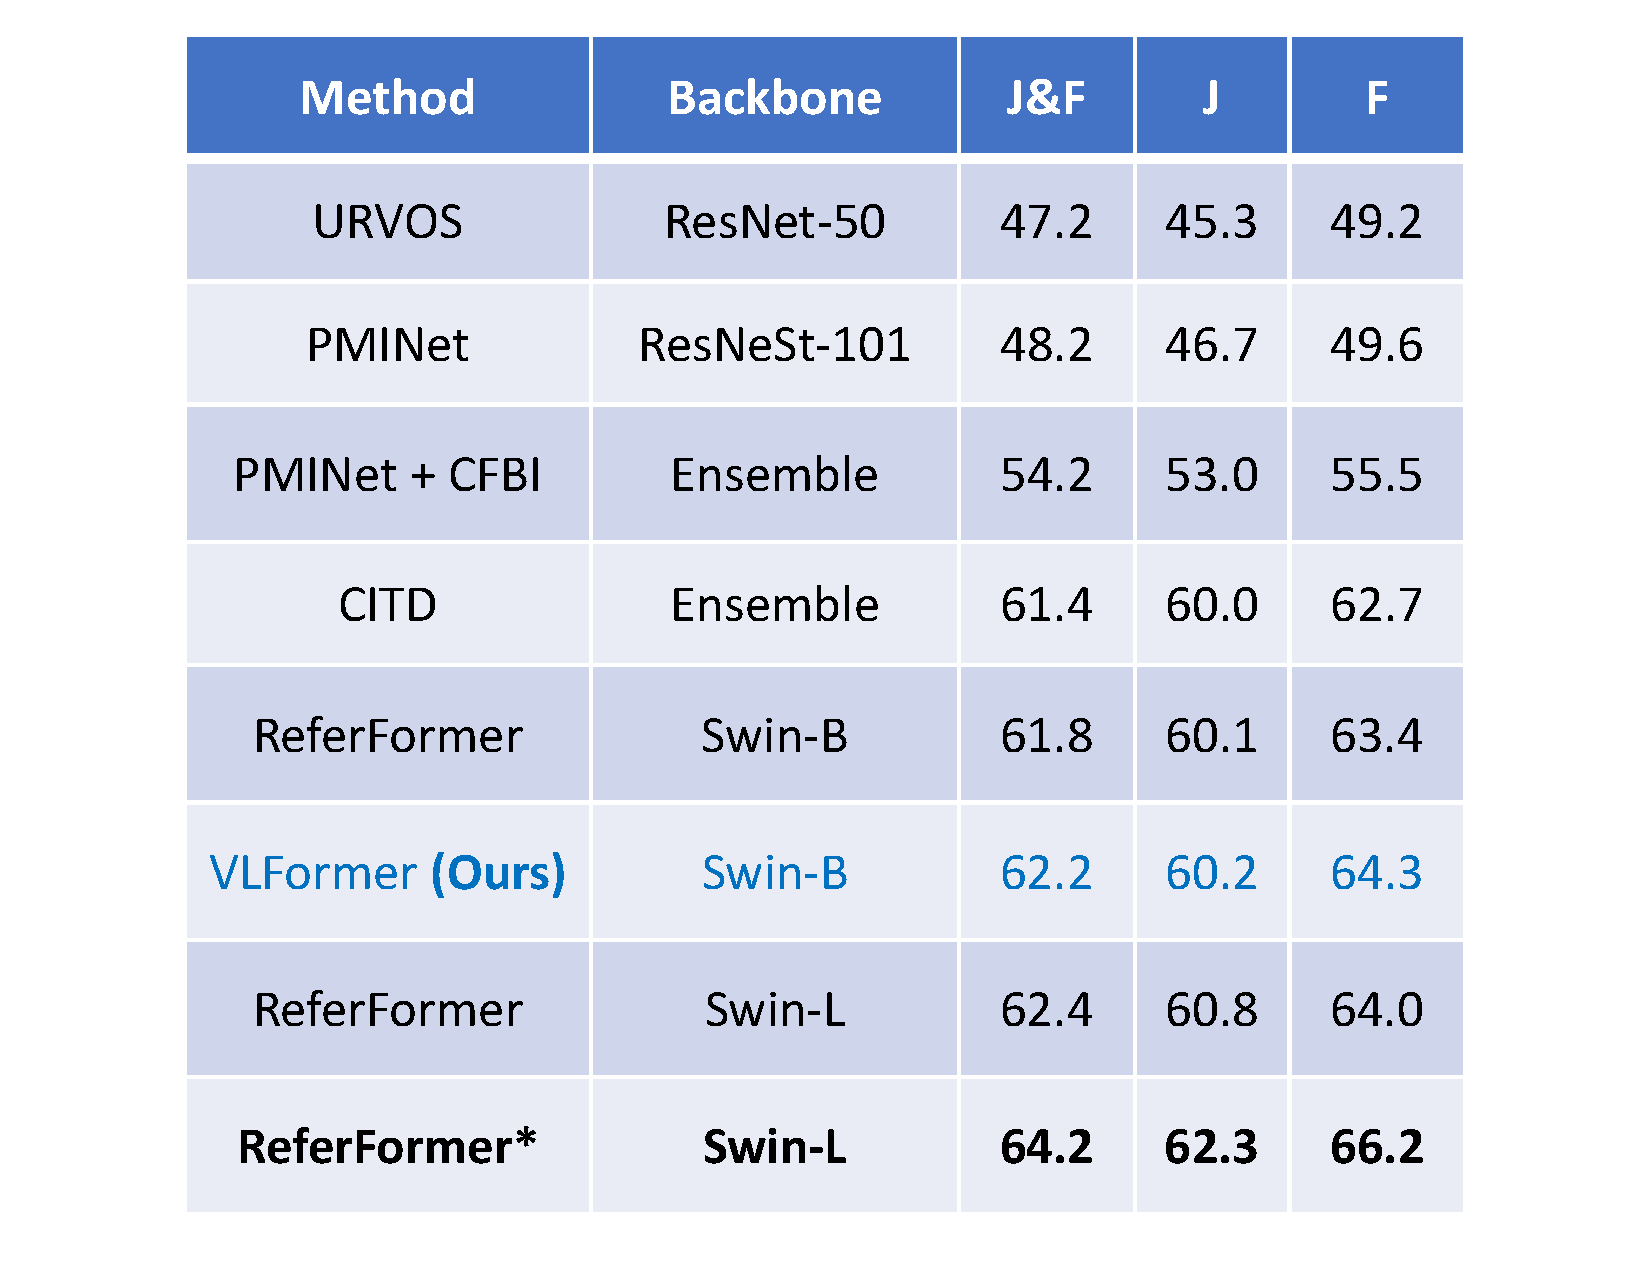
\includegraphics[width=\textwidth]{content/resources/images/referring_segmentation/RefYoutubeVOS2022-SOTA.pdf}
    \caption{Comparison with the state-of-the-art methods on Refer-Youtube-VOS development dataset. * means joint training with external datasets.}
    \label{tab:refyoutube2022_dev}
\end{table}


\begin{table}
\centering
% \resizebox{\linewidth}{!}{ %< auto-adjusts font size to fill line
\begin{tabular}{@{}clccc@{}}
\toprule
 & Team & $\mathcal{J\&F}(\uparrow)$ & $\mathcal{J}(\uparrow)$ & $\mathcal{F}(\uparrow)$ \\
\midrule
1 & Bo\_\_\_ & 0.641 & 0.622 & 0.661 \\
2 & jiliushi & 0.617 & 0.598 & 0.636 \\
3 & PENG & 0.608 & 0.589 & 0.627 \\
4 & ds-hohhot & 0.596 & 0.579 & 0.612 \\
5 & JQK & 0.594 & 0.577 & 0.611 \\
6 & nero(\textbf{Ours}) & 0.580 & 0.561 & 0.599\\
\bottomrule
\end{tabular}
% } % \resizebox
\caption{
% 
Results in Ref-YouTube-VOS 2022 \textit{test} set.
% 
} % \caption
\label{tab:refyoutube2022}
\end{table}

Table \ref{tab:refyoutube2022_dev} shows our results in the Refer-Youtube-VOS 2021 development set. The table also shows the comparison between our approach and state-of-the-art methods in the same datasets. Our approach achieves 62.2\% in overall ($\mathcal{J\&F}$) with 60.2\% and $64.3\%$ in $\mathcal{J}$ and $\mathcal{F}$, respectively. As we can see, we can surpass the previous competitive method with an ensemble technique and post-processing as PMINet + CFBI, CITD\cite{liang_rethinking_nodate} with a considerable margin of 8\% and 0.8\%. Compared to the current state-of-the-art ReferFormer\cite{wu_language_2022}, in the same backbone Swin-B, we slightly beat ReferFormer of 0.4\%. A larger backbone Swin-L in ReferFormer achieves just 62.4\% compared to 62.2\% of ours, and after joint training with external datasets, the results of ReferFormer Swin-L increase 1.8\% (from 62.4\% to 64.2\%) in overall. However, our method is still promising. Due to the lack of resources, we can not train our method with the same computational system as ReferFormer. We used only two 12GB VRAM RTX 2080 Ti instead of 8-16 NVIDIA Tesla V100 (32GB VRAM) as ReferFormer. 

Table \ref{tab:refyoutube2022} shows the leaderboard of the YouTubeVOS Challenge 2022 Track 3: Referring Video Object Segmentation on the testing set. The top 5 teams focused on heavy inference and post-processing, such as: Inference with multiple scales, multiple augmentations (flip horizontal, vertical,...), and multiple semi-supervised video object segmentation models for post-processing. Meanwhile, our team \citeown{nguyen_visual-language_2022} ranks 6th without just only one scale in inference and post-processing. No ensemble technique is used in our method.

\section{RefCOCO, RefCOCO+ and G-Ref}
\label{sec:ris_dataset}
\subsection{Dataset}
% The datasets were collected using the ReferitGame. In this two-player game, the first player is given an image with a segmented object and asked to write a language expression to describe the target object. The second one is shown only the image and the referring expression and asks to choose the corresponding object. 
% RefCOCO has 142,209 expressions for 50,000 objects in 19,994 images, and RefCOCO+ consists of 141,564 expressions for 49,856 objects in 19,992 images. 

We evaluate our VLFormer on three commonly used datasets for referring image segmentation: RefCOCO, RefCOCO+ and G-Ref.

\textbf{RefCOCO \& RefCOCO+} were collected using the two-player  ReferitGame. In this game, the first player is given an image with a segmented object and asked to write a language expression to describe the target object. The second one is shown only the image and the referring expression and asks to choose the corresponding object. 
RefCOCO has 142,209 expressions for 50,000 objects in 19,994 images, and RefCOCO+ consists of 141,564 expressions for 49,856 objects in 19,992 images. Some kinds of words, e.g., words about absolute locations, are not used in the RefCOCO+ dataset. Therefore, it is considered to be more challenging than the RefCOCO dataset. The expressions in RefCOCO and RefCOCO+ are very concise, contains 3.5 words on average, and tend to have more objects of the same category per image (3.9 on average).

\textbf{G-Ref} is another commonly widely used dataset. It contains 104,560 expressions referring to 54,822 objects belonging to 26,711 images. Compared to RefCOCO and RefCOCO+, the average sentence length in G-Ref dataset is longer (8.4 words on average), and G-Ref has a richer word usage. However, G-Ref has fewer objects of the same category per image than RefCOCO and RefCOCO+ (1.6 on average).

\subsection{Evaluation metrics}
There are two metrics we use for experiments: IoU and Precision@X. The IoU score shows the quality of the prediction overlapped with the ground-truth, which demonstrates the overall performance of the approach. The detail of this metric is described in the section \ref{sec:metric}. The Precision@X reports the successful referring rate at the threshold X of the IoU score, which focuses on the referring ability of the method.

% The common evaluation metric used in the RefCOCO and RefCOCO+ is the IoU score. The detail of this metric is described in the section \ref{sec:metric} 

% \subsection{Results}
\subsection{Comparison with State-of-the-art}

% \begin{table}[ht]
%     \centering
%     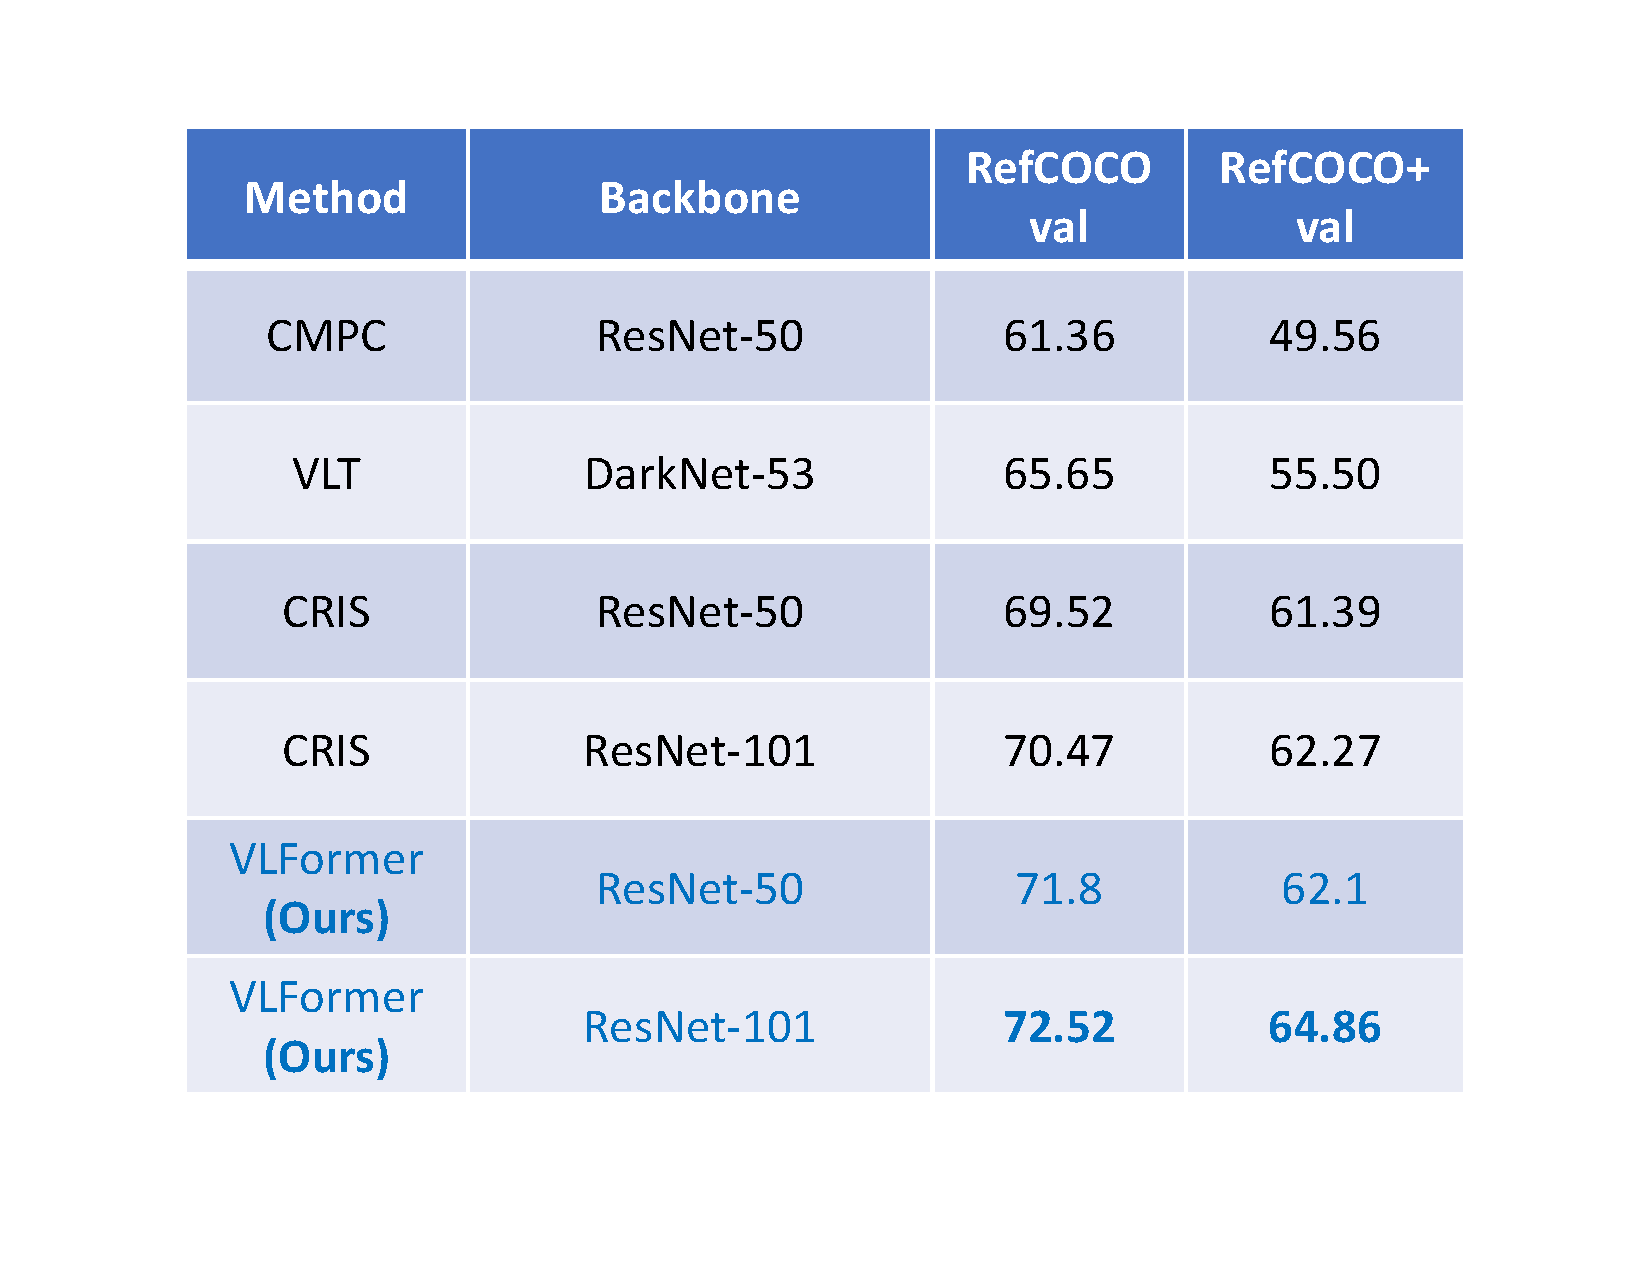
\includegraphics[width=\textwidth]{content/resources/images/referring_segmentation/RefCOCO-SOTA.pdf}
%     \caption{Comparison with the state-of-the-art methods on RefCOCO dataset.}
%     \label{tab:refcoco}
% \end{table}

 
\begin{table*}[ht]
\centering
\begin{tabular}{c|c|ccc|ccc}
\toprule

\multirow{2}{*}{Method} & \multirow{2}{*}{Backbone} & \multicolumn{3}{c|}{RefCOCO} & \multicolumn{3}{c}{RefCOCO+} \\ \cline{3-8} 
                        &                           & val      & testA   & testB   & val      & testA    & testB      \\ \midrule
MAttNet~\cite{yu_mattnet_2018}                    & ResNet-101                & 56.51    & 62.37   & 51.70   & 46.67    & 52.39    & 40.08          \\
NMTree~\cite{liu_learning_2019}                    & ResNet-101                & 56.59    & 63.02   & 52.06   & 47.40    & 53.01    & 41.56          \\
CMSA~\cite{ye_cross-modal_2019}                    & ResNet-101                & 58.32    & 60.61   & 55.09   & 43.76    & 47.60    & 37.89           \\
Lang2Seg~\cite{chen_referring_2019}                    & ResNet-101                & 58.90    & 61.77   & 53.81   & -    & -    & -            \\
CMPC~\cite{huang_referring_2020} & ResNet-101                & 61.36    & 64.53   & 59.64   & 49.56    & 53.44    & 43.23          \\
EFNet~\cite{feng_encoder_2021}                    & ResNet-101                & 62.76    & 65.69   & 59.67   & 51.50    & 55.24    & 43.01         \\
VLT~\cite{ding_vision-language_2021}                     & DarkNet-53                & 65.65    & 68.29   & 62.73   & 55.5     & 59.2     & 49.36     \\
ReSTR~\cite{kim_restr_2022}                   & ViT-B-16                  & 67.22    & 69.3    & 64.45   & 55.78    & 60.44    & 48.27       \\
CRIS~\cite{wang_cris_2022}                    & ResNet-101                & 70.47    & 73.18   & 66.1    & 62.27    & 68.08    & 53.68    \\
LAVT~\cite{yang_lavt_2022}                    & Swin-B                    & 72.73    & 75.82   & 68.79   & 62.14    & 68.38    & 55.1        \\ \midrule
VLFormer\textbf{(Ours)}                    & ResNet-50                    & 73.92    & 76.03   & \textbf{70.86}   & 64.02    & 69.74    & 55.04        \\ 
VLFormer\textbf{(Ours)}                     & ResNet-101                & \textbf{74.67}    & \textbf{76.8}    & 70.42   & \textbf{64.80}    & \textbf{70.33}    & \textbf{56.33}       \\
\bottomrule
\end{tabular}


\caption{Comparisons with the state-of-the-art approaches on RefCOCO and RefCOCO+ benchmarks. We report the results of our method with various visual backbones. IoU is used as the main metric, and  ``-'' shows that the result is not available. The best performance is marked in boldface.}
\label{tab:sota}
\end{table*}


\begin{table*}[ht]
\centering
\begin{tabular}{c|c|cc}
\toprule

\multirow{2}{*}{Method} & \multirow{2}{*}{Backbone} & \multicolumn{2}{c}{G-Ref} \\ \cline{3-4} 
                        &                           & val         & test        \\ \midrule
MAttNet~\cite{yu_mattnet_2018}                    & ResNet-101                   & 47.64           & 48.61          \\
NMTree~\cite{liu_learning_2019}                    & ResNet-101                & 46.59           & 47.88           \\
Lang2Seg~\cite{chen_referring_2019}                    & ResNet-101                  & 46.37           & 46.95           \\

VLT~\cite{ding_vision-language_2021}                     & DarkNet-53                 & 52.99       & 56.65       \\
ReSTR~\cite{kim_restr_2022}                   & ViT-B-16                    & 54.48       & -           \\
CRIS~\cite{wang_cris_2022}                    & ResNet-101                 & 59.87       & 60.36       \\
LAVT~\cite{yang_lavt_2022}                    & Swin-B                     & 61.24       & 62.09       \\ \midrule
VLFormer\textbf{(Ours)}                    & ResNet-50                    & 65.69       & 65.90       \\ 
VLFormer\textbf{(Ours)}                     & ResNet-101 & \textbf{66.77}       & \textbf{66.52}       \\
\bottomrule
\end{tabular}


\caption{Comparisons with the state-of-the-art approaches on G-Ref dataset. We report the results of our method with various visual backbones. IoU is used as the main metric, and  ``-'' shows that the result is not available. The best performance is marked in boldface.}
\label{tab:sota2}
\end{table*}
% We compare our proposed method, VLFormer, with several state-of-the-art methods on two commonly used datasets: RefCOCO and RefCOCO+. As illustrated in Table \ref{tab:refcoco}, our method surpasses other methods on all datasets even though we utilize the ResNet-50. 

% On the RefCOCO and RefCOCO+, our model with ResNet-101 backbone significant outperforms the state-of-the-art CRIS\cite{wang_cris_2022} by 2.05\% and 2.59\%, respectively. It shows that our VLFormer performs an impressive ability to gather cross-model information to perfectly segmenting the target object.   

% Our approach and Vision-Language Transformer(VLT)\cite{ding_vision-language_2021} also rely on Transformer, however a huge gap between our approach and VLT with around 7\% and 9\% for RefCOCO and RefCOCO+, respectively, which indicates that our model effectively utilizes the knowledge of CLIP Text Encoder and the query-based mechanism. 


We compare our proposed method with several state-of-the-art methods on three common datasets for referring image segmentation. As illustrated in Table \ref{tab:sota}, our method suppresses other methods on each split of all datasets with large margins. The experiments demonstrate our method can surpass the state-of-the-art in several split of datasets even though we leverage the ResNet-50 visual backbone\cite{he_deep_2016}. 

On the RefCOCO dataset, our model significant outperforms the state-of-the-art LAVT\cite{yang_lavt_2022} by 1.94\%, 0.98\% and 1.63\% on three splits, respectively even our ResNet-101 visual backbone instead of SwinTransformer-Base. 

Similarly, VLFormer achieves impressive performance gains of around 2\% than several state-of-the-art methods on each split of the more challenging RefCOCO+ dataset.

Besides, on the most challenging dataset G-Ref, which has longer and more complex expressions, our proposed VLFormer outperforms the previous state-of-the-art with wide margins of 4.97\% and 4.43\% on the validation and test subsets, respectively. As shown in Table \ref{tab:sota2}, the results demonstrate that our proposed approach has the powerful ability to understand long and complex sentences. 






\subsection{Implementation details}
% In the RefCOCO and RefCOCO+ dataset, we train the network for $10$ epochs using the AdamW optimizer with the initial learning rate $10^{−4}$. A factor of 0.1 decreases the learning rate at the $7^{th}$ epoch. We train the network with a small batch size of 8 on 2 NVIDIA RTX 2080Ti with 12GB GPU.

We implement our method in PyTorch and use the CLIP Text Encoder implementation from HuggingFace's Transformer library. The Text Encoder is frozen during the training stage. We choose the number of Visual-Linguistic Transformer layers is $L = 2$, which contains $6$ VLB layers in total. 
The common feature dimension is set to 256.
In the RefCOCO, RefCOCO+, and G-Ref dataset, we train the network for $100$K iterations using the AdamW optimizer with the initial learning rate $10^{−4}$. Then a factor of 0.1 decreases the learning rate at the $70$K-th iteration. The network is trained with a small batch size of 8 on 2 NVIDIA RTX 2080Ti with 12GB GPU VRAM.


% \textbf{Failure cases}
\subsection{Ablation study}
% \begin{table}[H]
%         \centering
%         \begin{tabular}{cc}
%             \hline
%             \textbf{Queries} & \textbf{IoU} \\ \hline
%             1                & 71.6             \\
%             5                & 72.52        \\
%             10               & 72.3         \\
%             20               & 71.9             \\ \hline
%         \end{tabular}
%     % \begin{minipage}{.4\textwidth}
%     %     \centering
%     %     \begin{tabular}{cc}
%     %         \hline
%     %         \textbf{Queries} & \textbf{IoU} \\ \hline
%     %         1                & 71.6             \\
%     %         5                & 72.52        \\
%     %         10               & 72.3         \\
%     %         20               & 71.9             \\ \hline
%     %     \end{tabular}
%     % \end{minipage}
%     % \begin{minipage}{.4\textwidth}
%     %   \centering
%     %     \begin{tabular}{cc}
%     %         \hline
%     %         \textbf{Queries} & \textbf{IoU} \\ \hline
%     %         1                &              \\
%     %         5                & 72.52        \\
%     %         10               &              \\
%     %         20               &              \\ \hline
%     %     \end{tabular}
%     % \end{minipage}
    
%     \caption{
%         % 
%         Ablation study on RefCOCO set. All the models are using ResNet-101 as visual backbone.
%         % 
%         } % \caption
%         \label{tab:refyoutube2022}
%   \end{table}
  

\begin{table*}[h]
\centering
\begin{tabular}{c|c|c|c|c|c|c}
\toprule
\multicolumn{1}{c|}{} & Prec@0.5 & Prec@0.6 & Prec@0.7 & Prec@0.8 & Prec@0.9 & IoU \\
\midrule
\multicolumn{7}{l}{\textbf{(a)} Number of Visual-Language Transformer layers $(L)$}                                                                                                                                                                                                             \\ \midrule
0                          & 79.67             & 76.60             & 71.77             & 61.89             & 33.36             & 70.21   \\
1                          & 83.27             & 80.56             & 76.43             & 66.81             & 37.78             & 73.45   \\
2                        & \textbf{83.82}             & \textbf{81.18}             & \textbf{76.84}             & \textbf{67.48}             & \textbf{37.89}             & \textbf{73.92}   \\ \midrule
\multicolumn{7}{l}{\textbf{(b)} Text Encoder model}                                                                                                                                                                                                     \\ \midrule
CLIP                      & \textbf{83.82}             & \textbf{81.18}             & \textbf{76.84}             & \textbf{67.48}             & \textbf{37.89}             & \textbf{73.92}   \\
BERT                       & 79.85             & 77.54             & 73.80             & 65.23             & 36.62             & 70.73   \\ \midrule
\multicolumn{7}{l}{\textbf{(c)}Language Guidance Module (LGM)}                                                                                                                                                                                          \\ \midrule
With LGM                  & \textbf{83.82}             & \textbf{81.18}             & \textbf{76.84}             & \textbf{67.48}             & \textbf{37.89}             & \textbf{73.92}   \\
W/o LGM                    & 73.93             & 71.26             & 67.42             & 58.81             & 33.14             & 65.19   \\ \midrule
\multicolumn{7}{l}{\textbf{(d)} Number of object queries $(N)$}                                                                                                                                                                                                             \\ \midrule
1                          & 82.47             & 78.85             & 73.34             & 62.90              & 33.31             & 72.59   \\
3                          & 83.19             & 80.31             & 75.60             & 65.97              & 36.41             & 73.18   \\
5                          & \textbf{83.82}             & \textbf{81.18}             & \textbf{76.84}             & \textbf{67.48}             & \textbf{37.89}             & \textbf{73.92}   \\
8                          & 82.12             & 79.44             & 75.03             & 65.89              & 36.28             & 72.47   \\
10                         & 82.77             & 80.29             & 75.98             & 66.52             & 36.27             & 73.04
 \\ \bottomrule
\end{tabular}
\caption{\textbf{Ablation Study on RefCOCO.} The experiments are based on ResNet-50 visual backbone and conducted on the validation split of RefCOCO. W/o LGM indicates that LGM is not used in the Cross-modal Pixel Decoder}
\label{tab:ablation}
\end{table*}
In this section, we perform extensive ablation studies on the validation set of RefCOCO to study the effect of core components in our model. All models are based on ResNet-50 visual backbone. The details analysis is as follows.

\textbf{Visual-Linguistic Transformer} Table \ref{tab:ablation}(a) reports the performance of our framework in various number of Visual-Linguistic Transformer layers. Without Visual-Linguistic Transformer Block(VLB) $(L = 0)$, the model uses directly initialized object queries to associate with the output from Cross-modal Pixel Decoder to generate the object segmentation. In this case, the object queries play a role as the fully-connected layer to perform a per-pixel segmentation since the object queries are not updated by either vision or language information. As illustrated in Table \ref{tab:ablation}, removing all VLB modules leads to a drop of $3.71\%$ in IoU metric and a drop of $4\%$ to $6\%$ in precision across five thresholds. The setting of $L = 1$ immediately improves the performance with an increase of $3.24\%$ in IoU. Then our VLFormer consistently increases the results with more Visual-Linguistic Transformer layers. These results illustrate the effectiveness of aggregating the visual and linguistic features with object queries via our proposed VLB module to enrich the object representation ability. We choose $L = 2$ as the default in our framework to keep it simple and efficient. 

\textbf{Text Encoder.}
Table \ref{tab:ablation}(b) shows that using BERT to extract linguistic features instead of CLIP Text Encoder leads to a drop of $3.19\%$ in IoU. In addition, the precision drops by $2\%$ to $4\%$ in all the thresholds from 0.5 to 0.9. These results demonstrate the benefit of exploiting the ability to interact with visual features using linguistic features extracted from the CLIP Text Encoder model.  

\textbf{Language Guidance Module(LGM).} In Table \ref{tab:ablation}(c), we compare the standard Pixel Decoder and the Cross-modal Pixel Decoder, which leverages the Language Guidance Module to re-weight multi-scale visual features by the linguistic features. The results show that Language Guidance Module provides more accurate segmentation by an improvement of around $8\%$ in IoU score and $4-10\%$ of precision in several thresholds. It indicates that guiding the visual features with the expression is essential in the referring segmentation.



\textbf{Number of Queries.}
To demonstrate the effectiveness of the query number $N$, we show our VLFormer's performance with several numbers of queries in Table \ref{tab:ablation}(d). Benefitting from the Visual-Linguistic Transformer Block design, all the initial object queries are learned to incorporate both linguistic and visual features robustly to find the referred object. More queries can help the model make judgments among potential instances, which could handle the similarity of objects in complicated scenes. 
The performance is highest at $N = 5$ and begins slightly decrease when the number of queries gets larger. The model needs to predict more with a more significant number of queries. However, only one object is referred to in each pair of images and expressions. Therefore, the reason to explain this decrease is that the model learns with only one positive sample and many negative samples simultaneously, which can confuse the model in the training phase. When $N = 1$, referring expression may be complicated and confuses the target object being referred to. For example, "On the left of a tree, a man is feeding his buffalo". The referred object is a man feeding his buffalo on the left of a tree. With only one object feature, we may not capture the right target. However, when we use $N = 5$, the model can also pay attention to multiple objects in this sentence ("a tree", "a man", or "his buffalo"...) and then depends on the confidence scores to decide which one is the referred object.





% We perform an ablation study on RefCOCO to study the effect of core components in our model.

% % \textbf{Components Analysis.} 
% % Visual-Linguistic Transformer Block \\ 
% % CLIP Text Encoder \\ 
% % PointRend \\ 
% \textbf{Number of queries.}


% Benefitting from the Visual-Linguistic Transformer Block design, all the initial object queries are learned to incorporate both linguistic and visual features robustly to find the referred object. More queries can help the model make judgment among candidate instances, which could handle the similarity of objects in complicated scenes. 
% The performance is highest at $N = 5$ and begins slightly decrease when the number of queries gets larger. The model needs to predict more with a more significant number of queries. However, only one object is referred to in each pair of video and expression. Therefore, the reason to explain the decrease is that the model learns with only one positive sample and a lot of negative samples simultaneously, which can confuse the model in the training phase. When $N = 1$, we can imagine that sometimes the referring expression is complicated and causes confusion about the target object being referred. For example, "On the left of a tree, a man is feeding his buffalo". The referred object is a man feeding his buffalo on the left of a tree. With only one object feature, we may not capture the right target. However, when we use $N = 5$, the model can also pay attention to multiple objects in this sentence ("a tree", "a man", or "his buffalo"...) and then depends on the confidence scores to decide which one is the referred object.


\section{Qualitative Analysis}
\label{sec:rvos_qualitative_analysis}
% \textbf{Visualization}

\begin{figure}[ht]
    \centering
    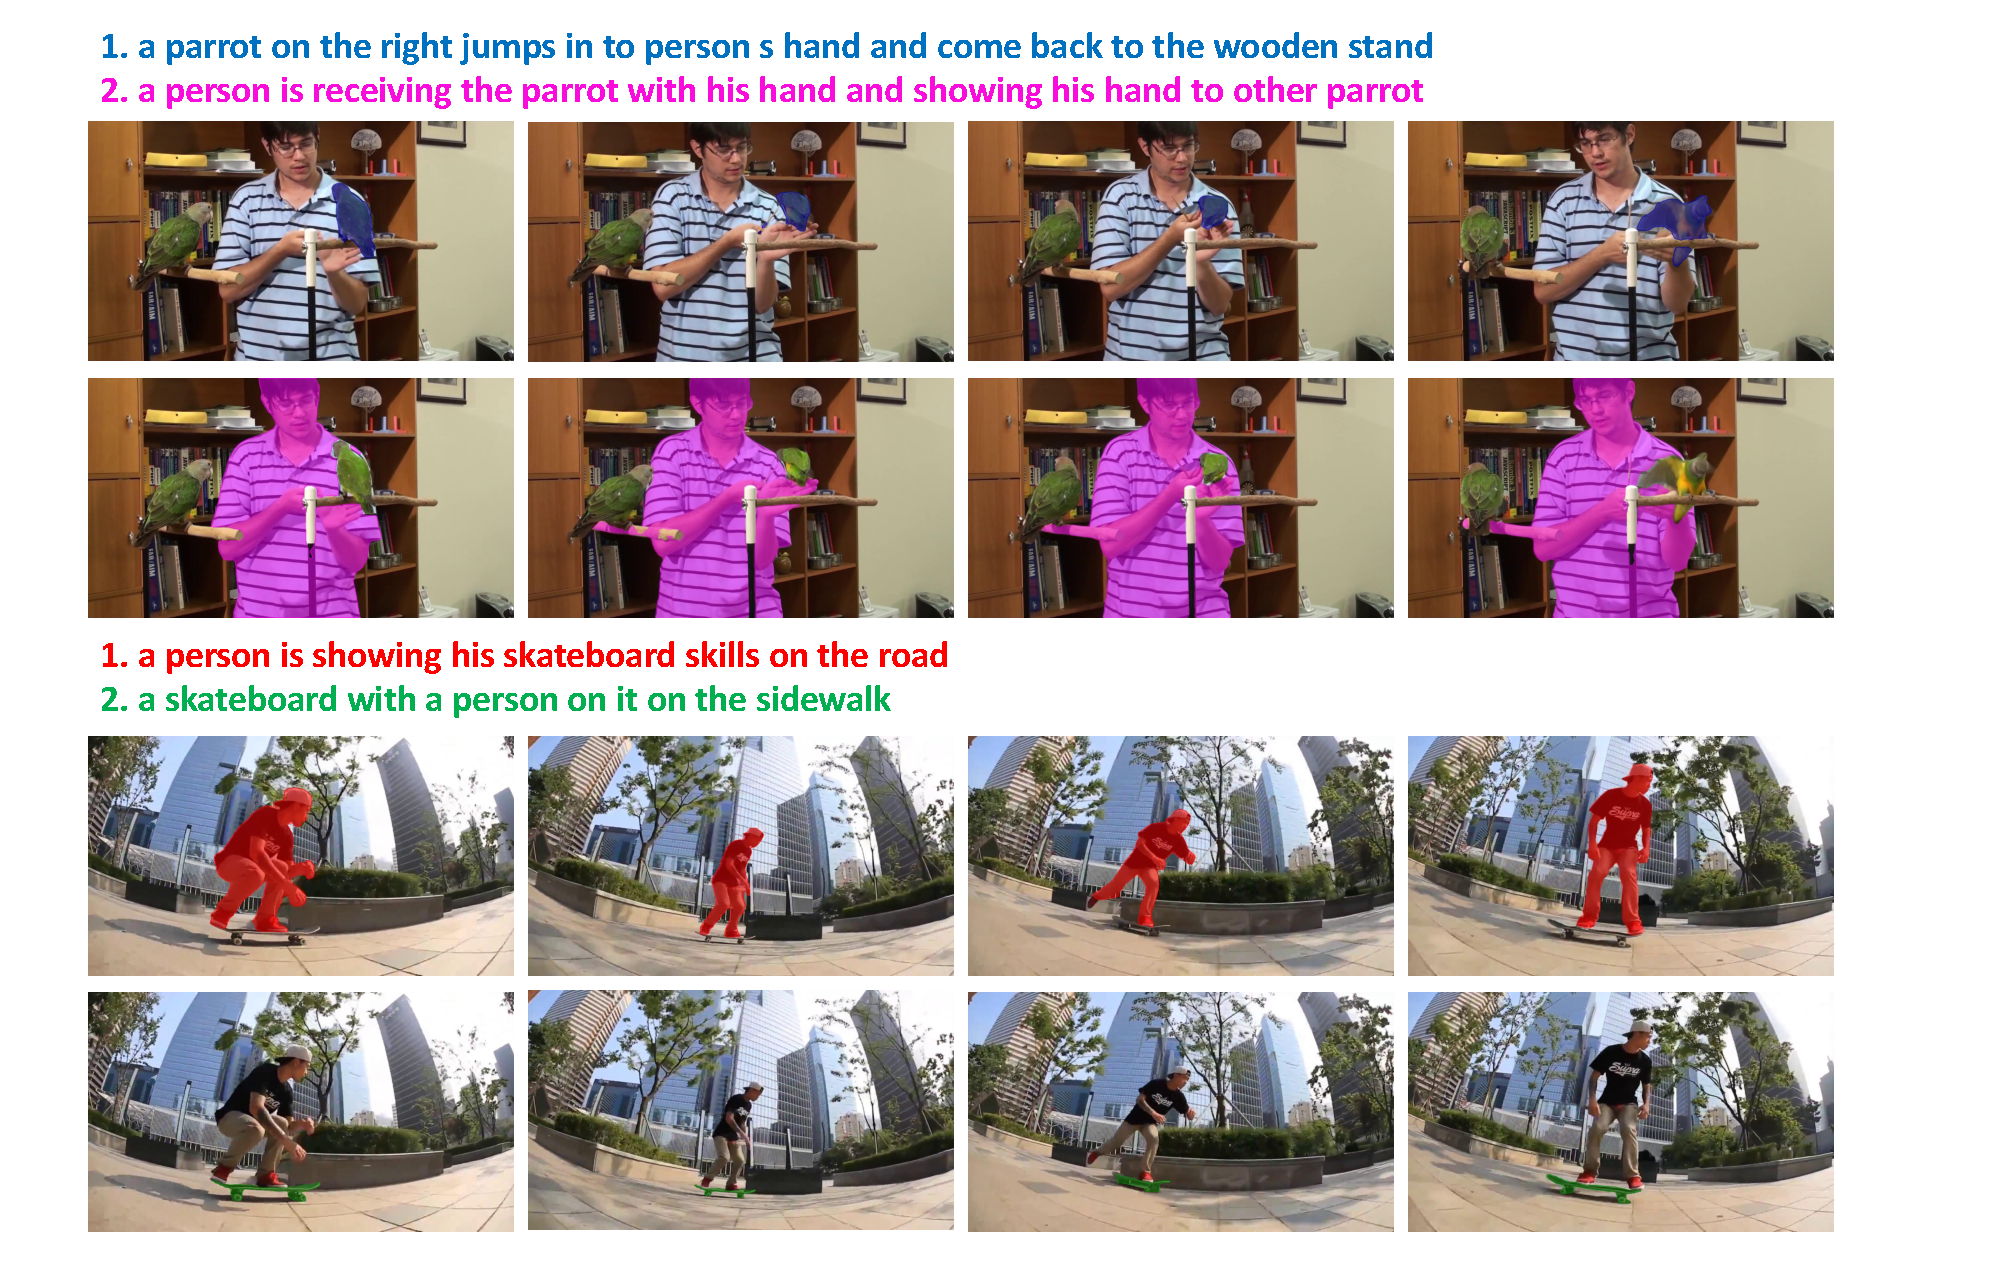
\includegraphics[width=\textwidth]{content/resources/images/referring_segmentation/QualitativeResults.pdf}
    \caption{\textbf{Qualitative results} on Refer-YouTube-VOS dataset. Each referring expression and the corresponding referred object are highlighted in the same color.}
    \label{fig:refyoutube_qualitative}
\end{figure}

Figure \ref{fig:refyoutube_qualitative} shows the qualitative results of our proposed model on the Refer-YouTube-VOS dataset. Each referring expression and the corresponding object are highlighted in the same color. The first two rows of images are about a video about a man standing with two parrots. The first expression \textit{"a parrot on the right jumps into person's hand and come back to the wooden stand"} describes the parrot on the right (blue color), and our model can segment almost perfectly. In the same video, the expression "a person is receiving the parrot with his hand and showing his hand to other parrot" refers to the man behind two parrots (pink color). Our model segments the person accurately except for the wooden stick nearby. 



\begin{figure*}[t]
    \centering
    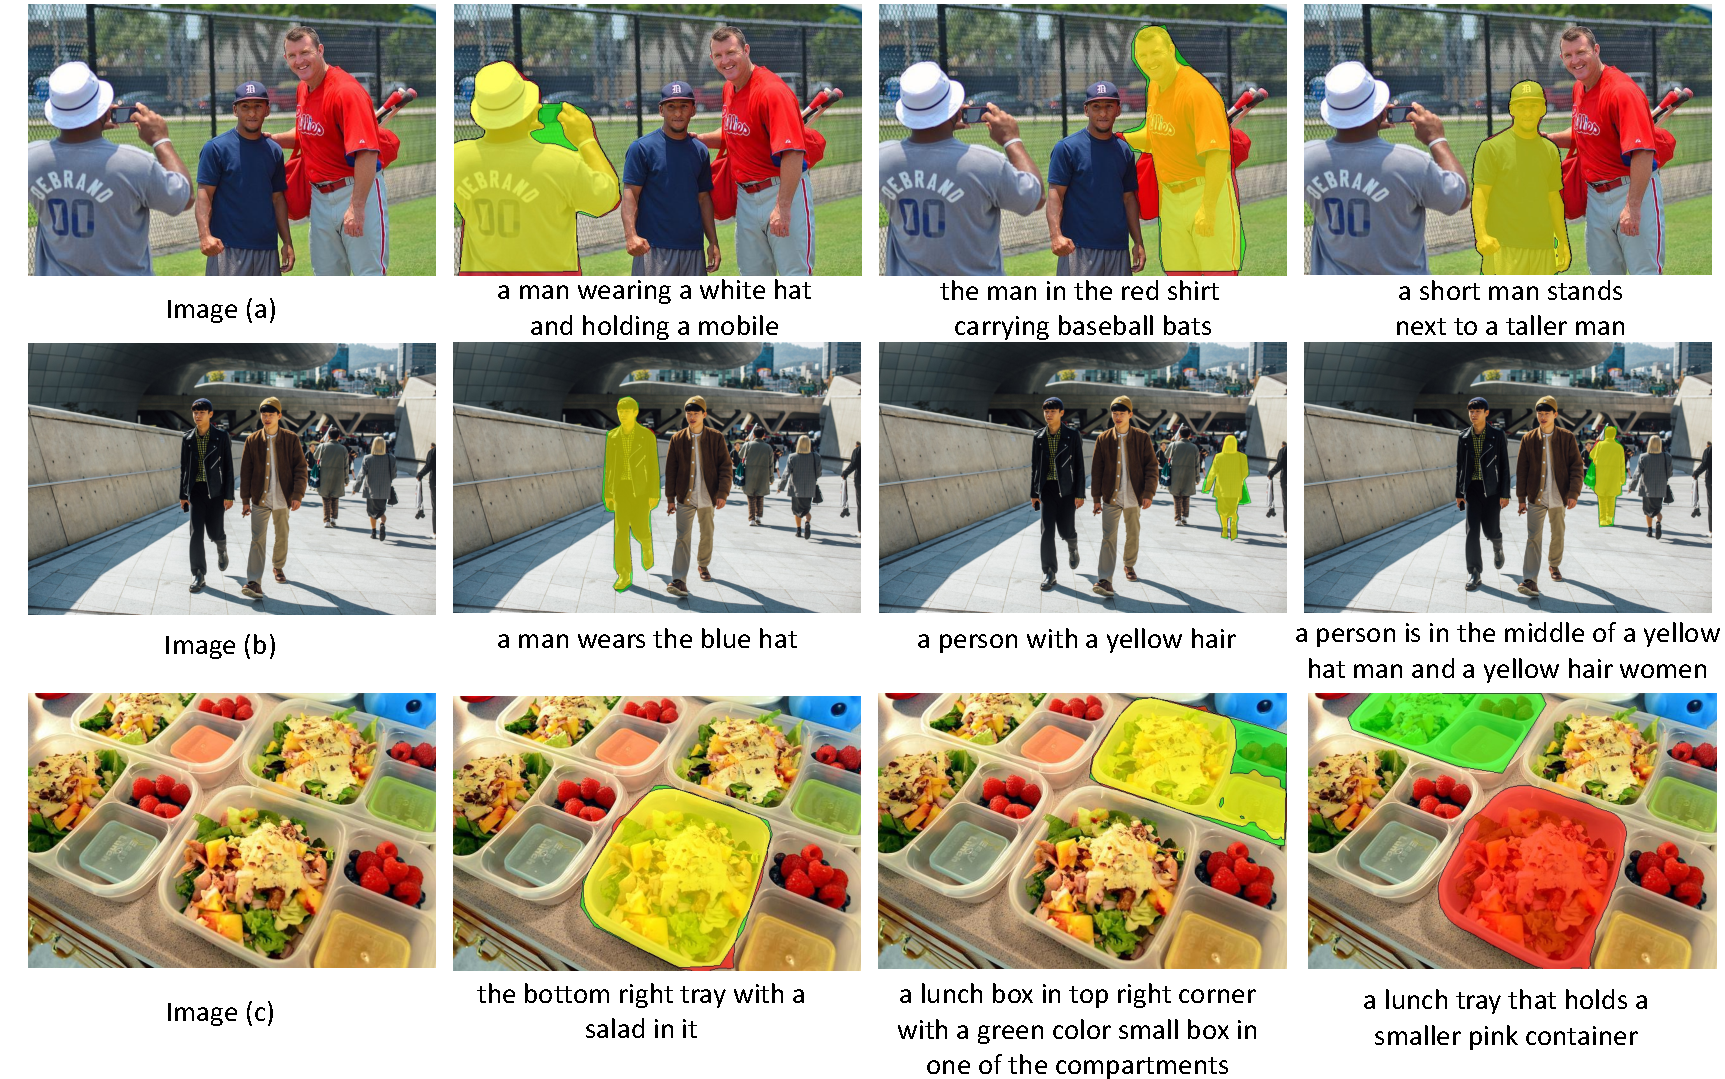
\includegraphics[width=0.8\textwidth]{content/resources/images/referring_segmentation/Visualization_New.pdf}
    \caption{The visualization of referring image segmentation results. From left to right: the input image, our overlaid results with the corresponding expressions. Overlaid color legend: green and red indicate the groundtruth and our segmentation results, respectively; while yellow highlights the intersection between the ground truth and our results.  }
    \label{fig:visualization}
\end{figure*}

We visualize the referring image segmentation results from our method in Figure \ref{fig:visualization}. To illustrate the impressive ability of our method, we show the predicting results of some examples with different expressions. Image (a) shows that our method can handle the expression containing the color information. The last image in the first row even demonstrates the capability to segment objects with attributes about the relative height, i.e., short, tall. In (b), we can see that our network can understand the color, i.e., blue, yellow and related stuff, i.e., hat, hair, and also identifies the referred person who locates in the middle of the two described objects. In (c), VLFormer correctly identifies the correct objects in the first two expressions. However, the third expression regarding the ``smaller pink container'' is confusing since there is no obvious pink container in the image. Therefore, VLFormer picks a pinkish object. This incorrect segmentation illustrates the failure case in our proposed work.

% Figure \ref{fig:visualization} also shows our model's ability to segment the referred object through a variety different target expressions. 

% \begin{figure}[ht]
%     \centering
%     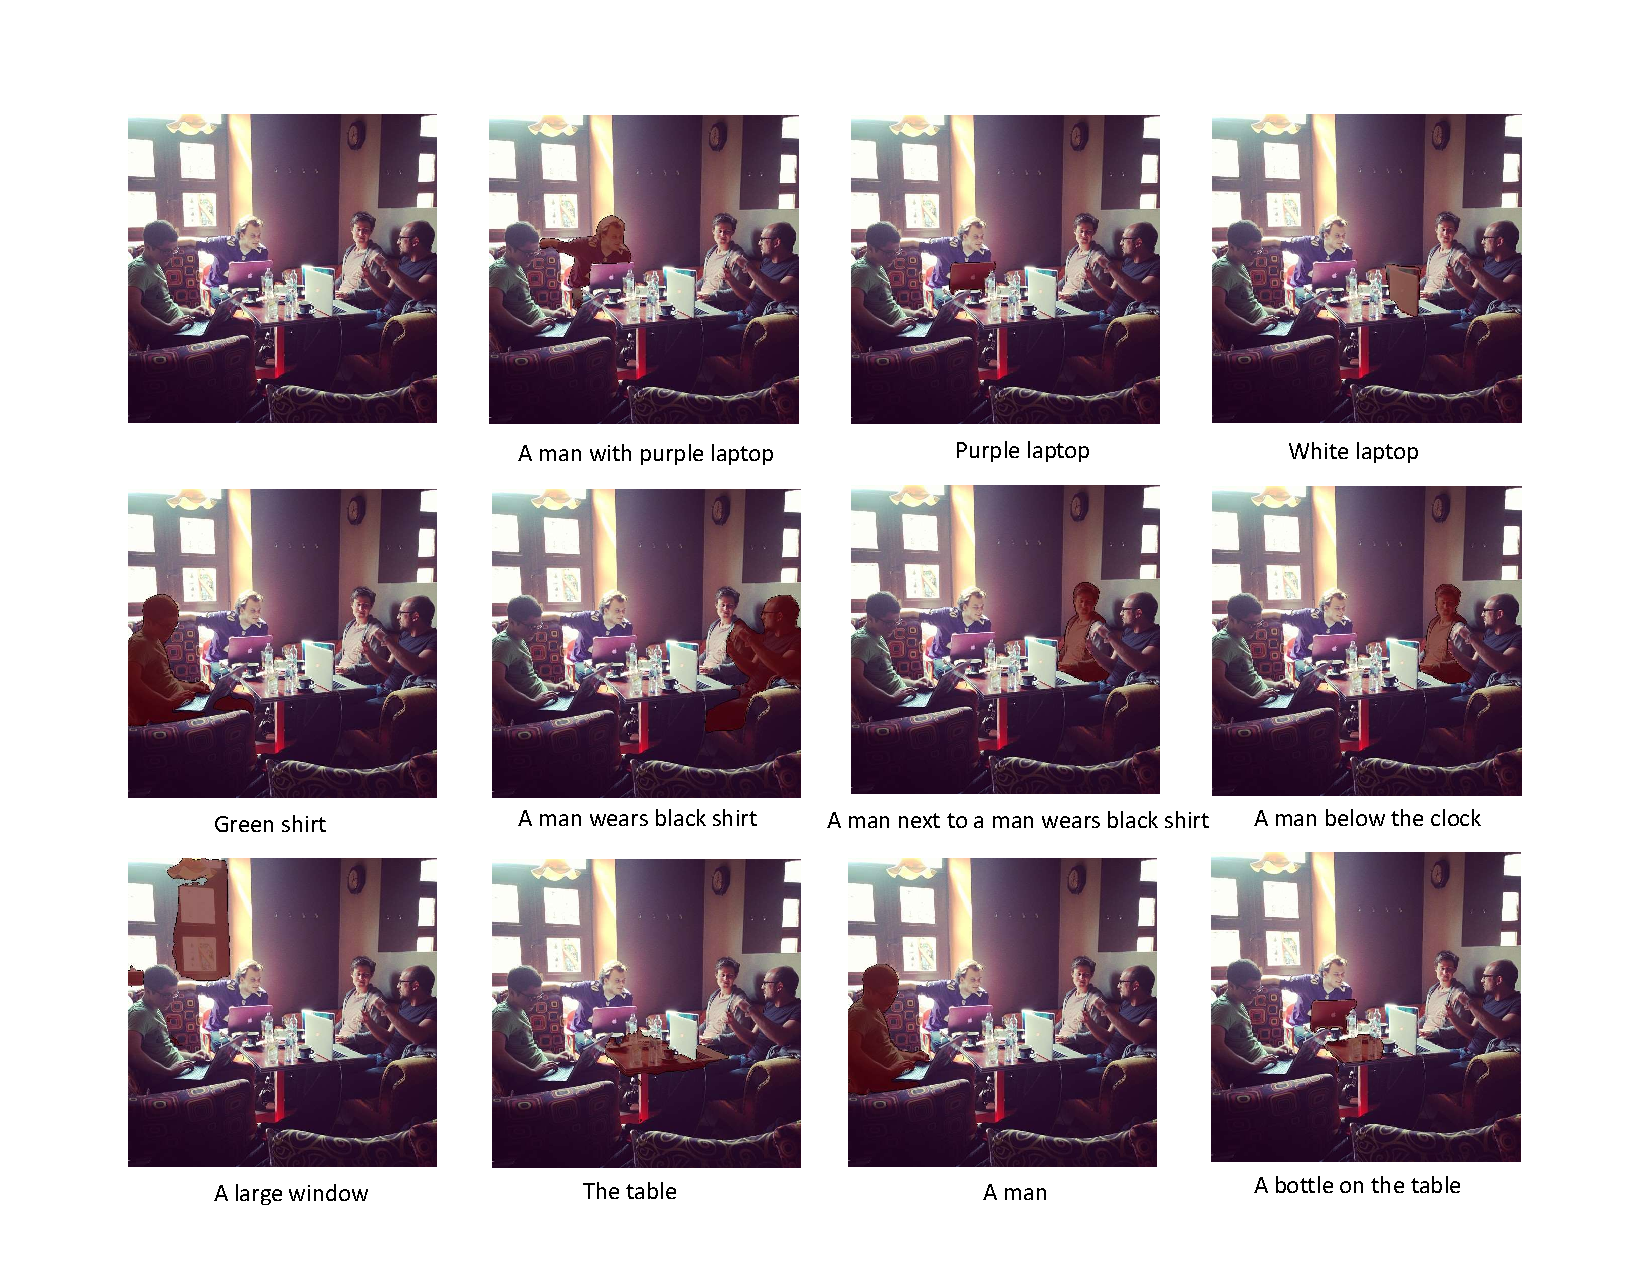
\includegraphics[width=\textwidth]{content/resources/images/referring_segmentation/Visualization.pdf}
%     \caption{Visualization. Diversity of referring expressions for an image. }
%     \label{fig:visualization}
% \end{figure}
